\section{Zielsetzung}
\label{sec:Zielsetzung}
In diesem Versuch soll die Bragg Bedingung überprüft, sowie das Emissionsspektrum der Cu-Röntgenröhre analysiert werden.
Zudem soll die Abschirmungskonstante für verschiedene Materialien bestimmt werden.

\section{Theorie}
\label{sec:Theorie}

\subsection{Erzeugung von Röntgenstrahlen}
\label{subsec:Erzeugung}

Zur Erzeugung werden in einer evakuierten Röhre Elektronen aus einer Glühkathode emittiert und auf eine Anode beschleunigt.
Durch das Auftreffen auf die Anode entstehen die Röntgenstrahlen, bestehend aus einem kontinuierlichen Bremsspektrum und
der spezifischen Röntgenstrahlen des Anodenmaterials.

\noindent
Bei der Abbremsung eines Elektrons im Coulombfeld des Atomkerns wird ein Photon bzw. Röntgenquant emittiert.
Die Energie dieses Photons ist gleich die, des abgebremsten Elektrons.
Dabei kann die Energie des Elektrons, sowie seine kinetische Energie an das Photon abgegeben werden.
Es folgt ein kontinuierliches Spektrum, das Bremsspektrum, siehe \autoref{fig:bremsspektrum}.
Kommt es zur vollständigen Abbremsung des Elektrons, wird die gesamte kinetische Energie in Strahlungsenergie umgewandelt.
Somit hat das Photon die größtmögliche Energie.

\noindent
Das Anodenmaterial kann so ioniesiert werden und ist in einer inneren Schale unterbesetzt.
Ein Elektron aus einer äußeren Schale kann nach emittieren eines Photons in die innere fallen.
Das Photon besitzt hierbei genau die Energiedifferenz zwischen den beiden Energienniveaus.
Somit wird das spezifische Spektrum mit scharfen Linien beschrieben.
Diese Energien sind dabei charakteristisch für das Anodenmaterial.

\begin{figure}
    \centering
    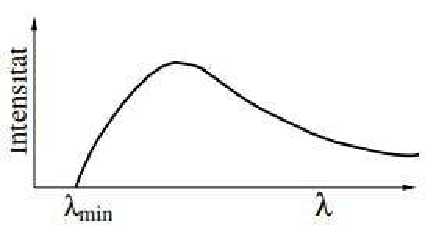
\includegraphics[width=\textwidth]{content/bremsspektrum.pdf}
    \caption{Das kontinuierliche Bremsspektrum.\cite{anleitung}}
    \label{fig:bremsspektrum}
\end{figure}

\subsection{Abschirmungskonstante}
\label{subsec:Abschirmungskonstante}

Bei einem Mehrelektronenatom kommt es zu einer Art Abschirmung der Kernladung durch die Hüllenelektronen und ihrer Wechselwirkung untereinander.
Die Coulomb-Anziehung ist somit geringer, es folgt für die Bindungsenergie $E_\text{n}$ eines Elektrons auf der n-ten Schale:

\begin{equation*}
    E_\text{n} = -R_{\infty} \cdot z^2_\text{eff} \cdot \frac{1}{n^2},
\end{equation*}

wobei für die effektive Kernladung $z_\text{eff} = z - \sigma$ gilt.
$\sigma$ steht hier für die Abschirmungskonstante und $R_\infty = \SI{13.6}{\electronvolt}$ für die Rydbergenergie.
$R_\infty$ ist dabei für jedes Elektron verschieden und wird empirisch bestimmt.
Zudem ist die Bindungsenergie auch nicht für alle äußeren Elektronen gleich, was an den Bahndrehimpulsen und Elektronenspins liegt.
Bei den charakteristischen Linien wird dies durch die Feinstruktur ersichtlich.
Eine Linie wird von mehreren, nah beieinander liegenden Linien unterteilt.
Die Aufspaltung der Linien ist aber in diesem Versuch nicht möglich.

\subsection{Absorption von Röntgenstrahlen}
\label{Absorption}

Der Comptoneffekt und der Photoeffekt treten vermehrt bei Röntgenstrahlung unter $\SI{1}{\mega\electronvolt}$ auf.
Mit größerwerdender Photonenenergie nimmt der Absorbtionskoeffizient ab.
Sobald die Energie die Bindungsenergie eines Elektrons aus der nächst inneren Schale überschritten hat, steigt der Koeffizient stark an.
Diese Absorptionskanten $\symup{h} \nu_\text{abs} = E_\text{n} - E_\infty$ gleichen sich sehr mit den der Bindungsenergie des Elektrons.
Unter Betrachtung der Feinstrucktur, wird die Bindungsenergie $E_\text{n,j}$ eines Elektrons mit der Sommerfeldschen Feinstruckturformel bestimmt:

\begin{equation}
    \label{eqn:sommerfeld}
    E_\text{n,j} = -R_\infty \cdot \Biggl( z^2_{\text{eff},1} \cdot \frac{1}{n^2} + \alpha^2 \cdot z^4_{\text{eff},2} \cdot \frac{1}{n^3} \cdot \Biggl(\frac{1}{j + \frac{1}{2}} - \frac{3}{4 \cdot n} \Biggr)\Biggr).
\end{equation}

Hier beschreibt $\alpha$ die Sommerfeldsche Feinstruckturkonstante, $\symup{n}$ die Hauptquantenzahl und $\symup{j}$ den Gesamdrehimpuls des Elektrons.
Mit der Gleichung \eqref{eqn:sommerfeld} kann die Abschirmkonstante $\sigma_\text{K,abs}$ eines Elektrons aus der K-Schale bestimmt werden:

\begin{equation}\label{eqn:absorptionskoeff}
    \sigma_K = z - \sqrt{\frac{E_K}{R_\infty} - \frac{\alpha^2 \cdot Z^4}{4}}
\end{equation}

Die Abschirmkonstante $\sigma_\text{L}$ kann mithilfe der Energiedifferenz $\increment E_\text{L} = E_\text{L}_{II} -E_\text{L}_{III}$ bestimmt werden.
Es gilt:

\begin{equation}
    \sigma_L = z -\Biggl( \frac{4}{\alpha} \cdot \sqrt{\frac{\increment E_L}{R_\infty} - \frac{5 \cdot \increment E_L}{R_\infty}} \Biggr)^{\frac{1}{2}}
                \cdot \Biggl(1 + \frac{19}{32} \cdot \alpha^2 \cdot \frac{\increment E_L}{R_\infty} \Biggr)^{\frac{1}{2}}
\end{equation}

Dabei ist $z$ die Ordungszahl.
Wird nun der Drehimpuls vernachlässigt, können die Abschirmkonstanten $\sigma_1, \sigma_2, \sigma_3$ für Kupfer wie folgt abgeschätzt werden:

\begin{align}
    \sigma_1 &= z - \sqrt{\frac{E_{K,\text{abs}}}{R_\infty}} \label{eq:sigma1} \\
    \sigma_2 &= z - 2 \cdot \sqrt{\frac{E_{K,\text{abs}} - E_{K, \alpha}}{R_\infty}} \label{eq:sigma2} \\
    \sigma_3 &= z - 3 \cdot \sqrt{\frac{E_{K,\text{abs}} - E_{K, \beta}}{R_\infty}} \label{eq:sigma3} 
\end{align}

\subsection{Bragg'sche Reflexion}
\label{subsec:Bragg}

Bei der Bragg'schen Reflexion fällt Rontgenlicht auf ein dreidimensionales Gitter.
Jedes Gitteratom sorgt für eine Beugung der Photonen.
Dadurch interferieren die Strahlen miteinander.
Konstruktive Interferenz passiert beim sogenannten Glanzwinkel $\theta$.
Ist die Gitterbreite $d$ bekannt, kann mit der Bragg'schen Bedingung, siehe Gleichung \eqref{eqn:BraggBedingung},
die Wellenlänge $\lambda$ der Röntgenstrahlung und somit die Energie $E$ bestimmt werden.

\begin{equation}
    \label{eqn:BraggBedingung}
    2 \cdot d \cdot \sin\theta = n \cdot \lambda
\end{equation}

\subsection{Moseley'sches Gesetz}
\label{subsec:moseley}
Um die Rydbergenergie $R_\infty$ zu bestimmen, wird das Moseley'sche Gesetz genutzt.
Demnach ist die Energie der $K_\alpha$-Strahlung proportional zu $z^2$, wobei $z$ die Kernladung ist.
Für $n = 1$ gilt:
\begin{equation}
    \label{eqn:moseley}
    E_K = R \cdot \symbol{h} \cdot (z - \sigma)^2
\end{equation}
$R$ ist hier die sogenannte Rydbergfrequenz.
Daraus folgt für die Rydbergenergie
\begin{equation}
    \label{eqn:rydbergenergie}
    R_\infty = R \cdot \symup{h}.
\end{equation}